

\begin{frame}{Estimation}
\begin{wideitemize}
\item Dynare is a great tool for estimation: It features many popular algorithms.
\item Estimation can be done with maximum likelihood (MLE) or Bayesian
\item More alternatives:
\begin{itemize}
    \item Calibration
    \item GMM
    \item Indirect inference
\end{itemize}
   \end{wideitemize}
\end{frame}

\begin{frame}{Our data for the NK model}
\begin{columns}[T]
\column{0.5\linewidth}
We download US data from FRED, corresponding to our basic New-Keynesian model.
\begin{wideenumerate}
\item The output gap $ygap = 100*\left(\log(y^{gdp})-\log(y^{pot})\right)$
\item Annualised nominal interest rates (federal funds rate)
\item Quarter-to-quarter inflation (GDP inflation)
\end{wideenumerate}
\column{0.5\linewidth}
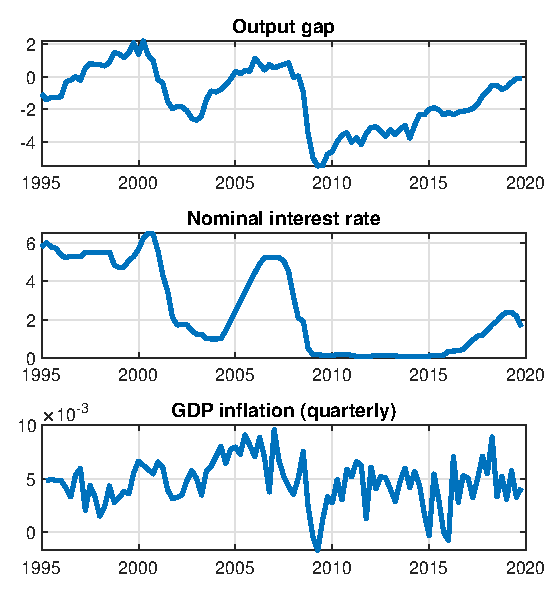
\includegraphics[width = 0.9\textwidth]{figures/dataplot.eps}
\end{columns}
\end{frame}


\begin{frame}{Linking model and data set}
\begin{wideitemize}
\item We extend the model with a set of \hi{observation equations} linking data and model variables.
\begin{itemize}
    \item Recall that all steady states are zero in our model (demeaned).
    \item One period corresponds to one quarter in the model.
    \item An amazing resource by Johannes Pfeifer: \href{https://drive.google.com/file/d/1r89OU5OE3CBa6tOlj6l3hNVWEaRH5Anv/view?usp=sharing}{A Guide to Specifying Observation Equations for the Estimation of DSGE Models}
\end{itemize}
\item Specify \hi{observed variables} after \texttt{varobs} command.
\item \hi{Declare dataset} via a \texttt{*.mat}-file or as an m-file
\begin{itemize}
    \item Example: \texttt{estimation(datafile=examplefile)}
\end{itemize}
\item Typically, the data feature a trend: Many options to deal with it!
\end{wideitemize}
\end{frame}

\begin{frame}[fragile]{Observation equations (cont'd)}
We need new variables and parameters (and calibrate the latter)
\begin{minted}{c++}
var
pieobs     ${\pi^{obs}}$ (long_name = 'Observed inflation')
ygapobs    ${y^{obs}}$   (long_name = 'Observed output gap')
inomobs    ${i^{obs}}$   (long_name = 'Observed nom. interest rate')
;

parameters
inomss   ${\bar{i}}$     (long_name = 'Mean interest rate')
piess    ${\bar{pi}}$    (long_name = 'Mean inflation')
;
\end{minted}
\end{frame}

\begin{frame}[fragile]{Observation equations (cont'd)}
\begin{minted}{c++}
model;

[name='Observation equation ygap']
ygapobs = y*100;

[name='Observation equation inflation (quarterly)']
pieobs = pie + piess;

[name='Observation equation interest rate']
inomobs = inom*400 + inomss;

end;
\end{minted}
\end{frame}




\begin{frame}{Why Bayesian?}
\begin{wideitemize}
\item Attractive underlying paradigm...
\item ...but for many macroeconomists its practicality
\item Avoids ``dilemma of absurd parameter estimates'' sometimes arising under pure maximum likelihood
\begin{itemize}
\item Structural parameter estimates at odds with outside evidence (e.g. from microfoundations).
\item Prior information can be brought it in: Macro time series sometimes not informative enough to discriminate among different theories
\end{itemize}
\item Model comparison is easy (even for non-nested models)
\item It's a system estimation method 
\end{wideitemize}
\end{frame}

\begin{frame}{Elements of Bayesian analysis}
\begin{wideitemize}
\item A Bayesian model consists of data $Y$ and parameters $\theta$ with a joint distribution $p(Y,\theta)$
\item \hi{Priors} contain information on parameters not included in the data: $p(\theta)$ (initial information independent of the data)
\item \hi{Likelihood} function based on the data: $L(Y,\theta)$
\begin{itemize}
    \item Likelihood of observing particular data $Y_{1:t}$ as a function of the parameters $\theta$.
    \item We are interested in finding $\theta$ that maximises the likelihood.
\end{itemize}
\item \hi{Posterior distribution} $p(\theta|Y)$ as a combination of prior and likelihood via Bayes theorem
\begin{itemize}
    \item This is a (potentially very complicated) probability distribution.
\end{itemize}
\end{wideitemize}
\end{frame}

\begin{frame}{Bayes theorem}
\begin{wideitemize}
\item Recall Bayes rule\footnote{Simply combine $p(A,B)=p(A|B)p(B)$ and $p(A,B)=p(B|A)p(A)$}
\begin{equation*}
     p(A|B) = \frac{p(B|A)p(A)}{p(B)}
\end{equation*}
\item In our case with $\theta$ as $A$ and the data $Y$ as $B$, we can define the \hi{posterior distribution} as 
\begin{equation*}
     p(\theta|Y) = \frac{L(Y,\theta)p(\theta)}{p(Y)} \propto L(Y,\theta)p(\theta)
\end{equation*}
\item $p(Y)$, the \hi{marginal data density}, is independent of the likelihood (probability of observing the data).
\begin{itemize}
    \item Can be used for model comparison.
\end{itemize}
\end{wideitemize}
\end{frame}

\begin{frame}{Specifying priors}
\begin{wideitemize}
\item Priors bring in \hi{information not included in the data}. They are random variables with probability distributions.
\item Can come from micro data, other papers, ...
\item Commonly used prior distributions:
\begin{itemize}
    \item \textit{Beta} distribution for parameters between 0 and 1 (e.g. shock persistence)
    \item \textit{Gamma} and \textit{Inverse Gamma} distributions for parameters restricted to be positive (e.g. shock standard deviation)
    \item \textit{Normal} distribution.
    \item \textit{Uniform} distribution.
\end{itemize}
\item Always check the plots to verify that your priors look sensible!
\item Simulate the model with the prior specification
\end{wideitemize}
\end{frame}

\begin{frame}[fragile]{Specifying priors: Example}
\begin{minted}{c++}
estimated_params;
rho_a,,,,BETA_PDF,0.8,0.1;
rho_c,,,,BETA_PDF,0.8,0.1;
rho_i,,,,BETA_PDF,0.5,0.1;
stderr u_a,INV_GAMMA_PDF,0.0025,2;
stderr u_c,INV_GAMMA_PDF,0.0025,2;
stderr u_i,INV_GAMMA_PDF,0.0025,2;
end;       
\end{minted}
\end{frame}

% \begin{frame}{Bayes theorem and the posterior}
% \begin{wideitemize}
% \item 
% \end{wideitemize}
% \end{frame}

\begin{frame}{Likelihood}
\begin{wideitemize}
\item For a given set of parameters $\theta$, we can solve the (linearised) model with Dynare and obtain a state space representation (more complex for OBCs):
\begin{equation*}
    X_t = T(\theta)X_{t-1} + C(\theta)u_t
\end{equation*}
\item Common problem: We rarely observe all variables in the data $Y_t$, formalised by the observation equation (here without measurement error)
\begin{equation*}
    Y_t = H(\theta)X_{t}
\end{equation*}
\item However, to evaluate the likelihood function, we need all model variables.
\item Key: Need to use a filter!
\end{wideitemize}
\end{frame}



\begin{frame}{Likelihood: Kalman filter}
\begin{wideitemize}
\item The Kalman filter is a very efficient recursive algorithm to construct the likelihood.
\item There must be at least as many shocks as observables to avoid stochastic singularity.
\item Full derivation in Hamilton's textbook.\footcite{hamilton2020time}
\item We will encounter the \hi{piecewise-linear Kalman filter} (PKF) later in more detail.
\end{wideitemize}
\end{frame}


   
\begin{frame}{Posterior}
\begin{wideitemize}
\item The posterior $p(\theta,Y)$ is a full distribution, typically not analytically tractable.
\item But we can easily get its value for a given parameter vector $\theta$
\item We can then use numerical methods to find the mode %(i.e. the value of $\theta$).
\item For further calculations, main problem: We cannot directly draw from the posterior distribution.
\item In general, however, we are interested in averages (expected values):
\begin{equation*}
    E\left[g(\theta|Y)\right] = \int g(\theta)p\left(\theta|Y\right)d\theta
\end{equation*}
\end{wideitemize}
\end{frame}

\begin{frame}{MCMC}
\begin{wideitemize}
\item Idea: Use \hi{Monte Carlo} integration by sampling $S$ draws from the posterior distribution
\begin{equation*}
    E\left[g(\theta|Y)\right] = \int g(\theta)p\left(\theta|Y\right)d\theta \approx \frac{1}{S}\sum_{s=1}^Sg(\theta_s)
\end{equation*}
\item Typically, we apply Markov Chain Monte Carlo Methods (MCMC), in particular the \hi{Metropolis-Hastings Algorithm}
\item The main idea: Efficiently explore the distribution! \texttt{mh\_jscale} allows you to target an acceptance rate (should be around 0.24).
\item MCMC generates (correlated) sequences \textit{as if} directly drawn from the $p(\theta,Y)$.
\item Need to check whether this is indeed the case using diagnostic tools. Dynare does this for you! See the manual.
\end{wideitemize}
\end{frame}


\begin{frame}{Posterior draws}
\begin{wideitemize}
\item Once we have obtained the posterior draws, we can do many interesting things!
\item We can calculate object reflecting parameter uncertainty:
\begin{itemize}
    \item IRFs (e.g. how much does inflation increase following a demand shocks?)
    \item Moments
    \item Welfare measures
    \item ...
\end{itemize}
\end{wideitemize}
\end{frame}
   


\begin{frame}{Estimation steps in a nutshell}
\begin{wideenumerate}
\item Specify a prior distribution.
    \item Evaluate the likelihood function using a Kalman filter
    \item Compute the posterior mode.
    \item Approximate the posterior distribution using Markov Chain Monte Carlo methods (MCMC)
    \item Based on the posterior distribution, compute objects of interest: moments, IRFs, parameter uncertainty,...
\end{wideenumerate}
For a textbook treatment: See Herbst and Schorheide\footcite{herbst2015bayesian}
\end{frame}


\begin{frame}[fragile]{Forecasts, filtered, and smoothed variables }
\begin{wideitemize}
\item Command \texttt{filtered} computes a forecast based on past information ($I_{t-1}$)
\begin{equation*}
    x_{t|t-1} = E\left[x_t|I_{t-1}\right]
\end{equation*}
\begin{itemize}
    \item Specify horizon using \texttt{filter\_step\_ahead = [4:8]}
\end{itemize}
\item Command \texttt{smoother} computes the posterior distribution of all endogenous variables and shocks using all available information up to period $T$
\begin{equation*}
    x_{t|T} = E\left[x_t|I_{T}\right]
\end{equation*}
\begin{itemize}
    \item Dynare also always produces smoothed shocks.  
\end{itemize}
\item Command \texttt{forecast} computes forecast of 10 periods.
\begin{minted}{c++}
estimation(filtered_vars,smoother,forecast=10)
\end{minted}
\end{wideitemize}
\end{frame}



\begin{frame}{Savings time load mode files and continuing a chain}
\begin{wideitemize}
\item Often, you can avoid re-doing some computations.
\item For example, you can use a previous mode file (automatically produced by Dynare).
\begin{itemize}
    \item Specify \texttt{mode\_file=filename\_mode}
    \item and skip re-computation: \texttt{mode\_compute=0}
\end{itemize}
\item Or continue a previous Markov chain using \texttt{load\_mh\_file}
\item Example: \texttt{estimation(mode\_file=filename\_mode, mode\_compute=0,
load\_mh\_file)}
\item You can run the chains in parallel: A significant speed up! \url{https://www.dynare.org/manual/the-configuration-file.html\#parallel-configuration}
\end{wideitemize}
\end{frame}

\begin{frame}[fragile]{Some checks before launching the estimation}
\begin{wideitemize}
\item Initialise the filter using the calibration
\begin{minted}{c++}
estimated_params_init(use_calibration);
end;
\end{minted}
\item Run a smoother based on calibration, e.g.
\begin{minted}{c++}
calib_smoother(datafile=mydatafile) 
y ygapobs inom inomobs pie pieobs;
\end{minted}
\item Triple check the units and frequency of your observed variables
\end{wideitemize}
\end{frame}




\begin{frame}[fragile]{Code for estimation}
\begin{minted}{c++}
estimation(
    //mh_replic=0, // Draws from the chain
    presample = 20,
    mh_nblocks=1,//number of chains
    use_univariate_filters_if_singularity_is_detected=0,
    datafile=dataobsnkm,
    nodisplay, 
    mh_jscale = 0.9,//tune the accept. ratio
    first_obs=2,
    graph_format=(eps,fig), 
    smoother);
\end{minted}
\end{frame}


% \begin{frame}{Shock decompositions}
% \begin{wideenumerate}
% \item TBD
% \end{wideenumerate}
% \end{frame}